\documentclass[aspectratio=169,11pt]{beamer}

\usepackage[australian]{babel}
\usepackage{amsmath}
\usepackage{amssymb}
\usepackage{array}
\usepackage{booktabs}
\usepackage{fontspec}
\usepackage{tikz}
\usepackage{xcolor}

\usetikzlibrary{arrows.meta,calc,fit,positioning,shapes.geometric}

\setsansfont{lmsans10-regular.otf}[
  BoldFont=lmsans10-bold.otf,
  ItalicFont=lmsans10-oblique.otf,
  BoldItalicFont=lmsans10-boldoblique.otf
]
\setmonofont{lmmono10-regular.otf}[
  BoldFont=lmmonolt10-bold.otf,
  ItalicFont=lmmono10-italic.otf
]

\definecolor{unswblue}{HTML}{1F2A44}
\definecolor{unswteal}{HTML}{007D7E}
\definecolor{unsworange}{HTML}{B35C16}
\definecolor{softblue}{HTML}{EAF0F7}
\definecolor{softteal}{HTML}{E5F4F3}
\definecolor{softorange}{HTML}{F8EDE5}
\definecolor{softgrey}{HTML}{F3F4F6}
\definecolor{darkgrey}{HTML}{394150}
\definecolor{logicgreen}{HTML}{557A46}

\usetheme{default}
\setbeamertemplate{navigation symbols}{}
\setbeamertemplate{footline}[frame number]
\setbeamercolor{title}{fg=unswblue}
\setbeamercolor{frametitle}{fg=unswblue}
\setbeamercolor{structure}{fg=unswteal}
\setbeamerfont{title}{series=\bfseries,size=\Large}
\setbeamerfont{subtitle}{size=\normalsize}
\setbeamerfont{frametitle}{series=\bfseries,size=\large}
\setbeamerfont{footline}{size=\scriptsize}

\setlength{\parskip}{0.35em}
\setlength{\tabcolsep}{5pt}

\newcommand{\minihead}[1]{\textbf{\color{unswblue}#1}}
\newcommand{\term}[1]{\textbf{\color{unswteal}#1}}
\newcommand{\activity}{\textbf{\color{unsworange}Large-class checkpoint}}
\newcommand{\choice}[2]{\textbf{#1.} #2}
\newcommand{\source}[1]{\vfill{\scriptsize\color{darkgrey}Source basis: #1}}
\newcommand{\lit}[1]{\texttt{#1}}
\newcommand{\model}[1]{\{#1\}}

\newcommand{\conceptbox}[3]{%
  \begin{tikzpicture}
    \node[
      draw=#1,
      fill=#1!8,
      rounded corners=3pt,
      inner sep=7pt,
      text width=#2,
      align=left
    ] {#3};
  \end{tikzpicture}
}

\newcommand{\clausebox}[2]{%
  \tikz[baseline=(x.base)]\node[
    draw=#1,
    fill=#1!8,
    rounded corners=2pt,
    inner xsep=5pt,
    inner ysep=3pt,
    font=\small
  ] (x) {$#2$};%
}

\title{Knowledge Representation}
\subtitle{Propositional logic, inference, and resolution}
\author{COMP9414 Artificial Intelligence}
\date{Week 3}

\begin{document}

\begin{frame}
  \titlepage
\end{frame}

\begin{frame}{What This 3-Hour Class Is For}
  \begin{columns}[T,onlytextwidth]
    \begin{column}{0.48\textwidth}
      \minihead{Students should leave able to}
      \begin{itemize}
        \item read propositional formulas as constraints on possible worlds;
        \item explain entailment using models;
        \item distinguish semantic truth from syntactic proof;
        \item convert small formulas to CNF;
        \item use resolution refutation on a small example.
      \end{itemize}
    \end{column}
    \begin{column}{0.48\textwidth}
      \minihead{Pacing}
      \begin{tabular}{p{0.22\linewidth}p{0.66\linewidth}}
        0:00 & Logic as a representation language \\
        0:25 & Syntax, semantics, models, entailment \\
        1:10 & Horn clauses and chaining \\
        1:35 & Break \\
        1:45 & CNF, satisfiability, refutation \\
        2:15 & Resolution proof method \\
        2:45 & Why propositional logic is limited \\
      \end{tabular}
    \end{column}
  \end{columns}
\end{frame}

\begin{frame}{Source Backbone}
  \small
  \begin{tabular}{>{\bfseries}p{0.28\linewidth}p{0.62\linewidth}}
    \toprule
    Section & Local source material used \\
    \midrule
    Logical agents & AIMA chapter 7, \texttt{chapter07.pdf} \\
    Propositional basics & Berkeley CS188 lecture 8, \texttt{cs188-sp24-lec08.pdf}; CS221 syntax/semantics PDFs \\
    Entailment and inference & Berkeley CS188 lecture 8; AIMA chapter 7; CS221 inference rules \\
    Horn clauses & AIMA chapter 7; CS221 modus ponens PDF \\
    CNF and satisfiability & Berkeley CS188 lecture 8; AIMA chapter 7; Stanford/CS221 resolution PDF \\
    Resolution refutation & Stanford/CS221 resolution PDF; Basel handout; TUM resolution slides \\
    FOL preview & AIMA chapter 7 summary point, adapted as a short bridge \\
    \bottomrule
  \end{tabular}

  \vspace{0.8em}
  The deck is not a clone of any source deck. It is a new Beamer lecture built from the local source pack.
\end{frame}

\begin{frame}{Large-Class Rhythm}
  \begin{columns}[T,onlytextwidth]
    \begin{column}{0.48\textwidth}
      \minihead{Every block has}
      \begin{itemize}
        \item a small formal idea;
        \item one concrete model or clause example;
        \item a silent A-D checkpoint;
        \item a short answer slide.
      \end{itemize}
    \end{column}
    \begin{column}{0.48\textwidth}
      \minihead{Why}
      \begin{itemize}
        \item Logic is easy to make too abstract.
        \item Checkpoints keep students evaluating formulas themselves.
        \item The resolution proof is built in layers.
        \item FOL is only a preview, not the main event.
      \end{itemize}
    \end{column}
  \end{columns}
\end{frame}

\section{Logical Agents}

\begin{frame}{Why Logic Enters AI}
  \begin{columns}[T,onlytextwidth]
    \begin{column}{0.47\textwidth}
      \minihead{Search gave us}
      \begin{itemize}
        \item states;
        \item actions;
        \item paths;
        \item cost and heuristic estimates.
      \end{itemize}
    \end{column}
    \begin{column}{0.49\textwidth}
      \minihead{Logic adds}
      \begin{itemize}
        \item explicit facts about a world;
        \item rules that connect facts;
        \item queries about what must be true;
        \item proof methods that derive new information.
      \end{itemize}
    \end{column}
  \end{columns}

  \source{AIMA chapter 7; Berkeley CS188 lecture 8.}
\end{frame}

\begin{frame}{Knowledge-Based Agent Pattern}
  \begin{center}
    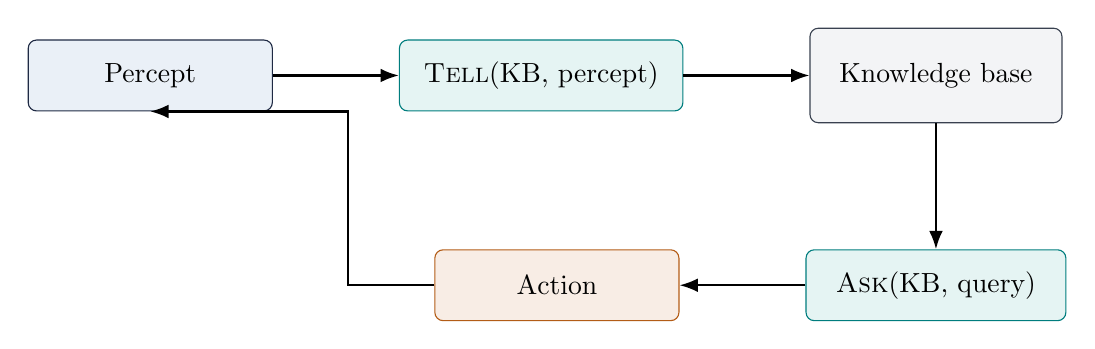
\begin{tikzpicture}[node distance=1.6cm,>=Latex]
      \node[draw=unswblue,fill=softblue,rounded corners=3pt,minimum width=3.1cm,minimum height=0.9cm] (percept) {Percept};
      \node[draw=unswteal,fill=softteal,rounded corners=3pt,minimum width=3.6cm,minimum height=0.9cm,right=of percept] (tell) {\textsc{Tell}(KB, percept)};
      \node[draw=darkgrey,fill=softgrey,rounded corners=3pt,minimum width=3.2cm,minimum height=1.2cm,right=of tell] (kb) {Knowledge base};
      \node[draw=unswteal,fill=softteal,rounded corners=3pt,minimum width=3.3cm,minimum height=0.9cm,below=of kb] (ask) {\textsc{Ask}(KB, query)};
      \node[draw=unsworange,fill=softorange,rounded corners=3pt,minimum width=3.1cm,minimum height=0.9cm,left=of ask] (action) {Action};

      \draw[->,thick] (percept) -- (tell);
      \draw[->,thick] (tell) -- (kb);
      \draw[->,thick] (kb) -- (ask);
      \draw[->,thick] (ask) -- (action);
      \draw[->,thick] (action.west) -- ++(-1.1,0) |- (percept.south);
    \end{tikzpicture}
  \end{center}

  \begin{itemize}
    \item \textsc{Tell}: add percepts and action records.
    \item \textsc{Ask}: derive what action or hidden fact follows from the KB.
    \item The inference engine should be domain-independent; the KB contains the domain content.
  \end{itemize}

  \source{AIMA chapter 7, knowledge-based agent slides.}
\end{frame}

\begin{frame}{A Small Running Domain}
  \begin{columns}[T,onlytextwidth]
    \begin{column}{0.48\textwidth}
      \minihead{Office robot}
      \begin{itemize}
        \item The robot observes whether a door is locked.
        \item A keycard opens the lab.
        \item The parcel should end in the lab.
        \item Some facts are directly observed; others must be inferred.
      \end{itemize}
    \end{column}
    \begin{column}{0.48\textwidth}
      \minihead{Example symbols}
      \begin{align*}
        K &: \text{robot has keycard}\\
        L &: \text{lab door is locked}\\
        P &: \text{robot has parcel}\\
        D &: \text{parcel delivered}\\
        S &: \text{safe to enter lab}
      \end{align*}
    \end{column}
  \end{columns}
\end{frame}

\begin{frame}{The Kind Of Question Logic Answers}
  \begin{columns}[T,onlytextwidth]
    \begin{column}{0.48\textwidth}
      \minihead{Knowledge base}
      \begin{align*}
        K &\rightarrow \neg L\\
        \neg L &\rightarrow S\\
        P \land S &\rightarrow D\\
        K\\
        P
      \end{align*}
    \end{column}
    \begin{column}{0.48\textwidth}
      \minihead{Query}
      \[
        KB \models D \; ?
      \]

      Read this as:

      \medskip
      In every possible world where the KB is true, is $D$ also true?
    \end{column}
  \end{columns}
\end{frame}

\section{Syntax And Semantics}

\begin{frame}{Three Levels To Keep Separate}
  \begin{center}
    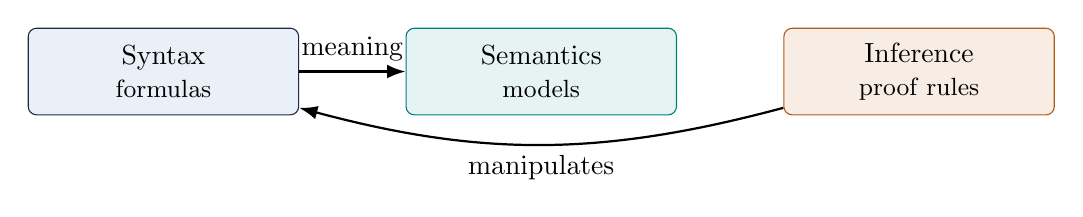
\begin{tikzpicture}[node distance=1.35cm,>=Latex]
      \node[draw=unswblue,fill=softblue,rounded corners=3pt,text width=3.2cm,align=center,minimum height=1.1cm] (syntax) {Syntax\\\small formulas};
      \node[draw=unswteal,fill=softteal,rounded corners=3pt,text width=3.2cm,align=center,minimum height=1.1cm,right=of syntax] (sem) {Semantics\\\small models};
      \node[draw=unsworange,fill=softorange,rounded corners=3pt,text width=3.2cm,align=center,minimum height=1.1cm,right=of sem] (rules) {Inference\\\small proof rules};
      \draw[->,thick] (syntax) -- node[above]{meaning} (sem);
      \draw[->,thick] (rules) to[bend left=15] node[below]{manipulates} (syntax);
    \end{tikzpicture}
  \end{center}

  \begin{itemize}
    \item Syntax says which strings are legal formulas.
    \item Semantics says when formulas are true in a model.
    \item Inference rules derive new formulas from old formulas.
  \end{itemize}

  \source{CS221 syntax, semantics, and inference-rule slides; AIMA chapter 7.}
\end{frame}

\begin{frame}{Propositional Syntax}
  \begin{columns}[T,onlytextwidth]
    \begin{column}{0.45\textwidth}
      \minihead{Atomic propositions}
      \[
        A,\; B,\; C,\; Rain,\; Wet,\; DoorLocked
      \]

      Each is either true or false in a model.
    \end{column}
    \begin{column}{0.51\textwidth}
      \minihead{Connectives}
      \begin{tabular}{lll}
        \toprule
        Symbol & Name & Read as \\
        \midrule
        $\neg f$ & negation & not $f$ \\
        $f \land g$ & conjunction & $f$ and $g$ \\
        $f \lor g$ & disjunction & $f$ or $g$ \\
        $f \rightarrow g$ & implication & if $f$, then $g$ \\
        $f \leftrightarrow g$ & biconditional & $f$ iff $g$ \\
        \bottomrule
      \end{tabular}
    \end{column}
  \end{columns}

  \source{CS221 propositional syntax; Berkeley CS188 lecture 8.}
\end{frame}

\begin{frame}{Truth Conditions}
  \small
  \begin{center}
    \begin{tabular}{cc|ccccc}
      \toprule
      $f$ & $g$ & $\neg f$ & $f \land g$ & $f \lor g$ & $f \rightarrow g$ & $f \leftrightarrow g$ \\
      \midrule
      F & F & T & F & F & T & T \\
      F & T & T & F & T & T & F \\
      T & F & F & F & T & F & F \\
      T & T & F & T & T & T & T \\
      \bottomrule
    \end{tabular}
  \end{center}

  \vspace{0.8em}
  The implication row that surprises students is:

  \[
    F \rightarrow T = T
    \qquad
    F \rightarrow F = T
  \]

  A false premise does not violate an if-then claim.
\end{frame}

\begin{frame}{Parsing A Formula}
  \[
    ((\neg A \lor B) \rightarrow \neg(D \lor E)) \land (C \leftrightarrow C)
  \]

  \begin{columns}[T,onlytextwidth]
    \begin{column}{0.48\textwidth}
      \minihead{The formula is built recursively}
      \begin{itemize}
        \item $A,B,C,D,E$ are atomic formulas.
        \item $\neg A$ and $\neg(D \lor E)$ are formulas.
        \item $(\neg A \lor B) \rightarrow \neg(D \lor E)$ is a formula.
        \item The whole sentence is a conjunction.
      \end{itemize}
    \end{column}
    \begin{column}{0.48\textwidth}
      \minihead{Meaning comes later}
      \begin{itemize}
        \item Syntax alone does not tell us whether it is true.
        \item Truth requires a model: a truth assignment to each symbol.
      \end{itemize}
    \end{column}
  \end{columns}
\end{frame}

\begin{frame}{Checkpoint: Evaluate The Formula}
  \activity

  \vspace{0.6em}
  Model:
  \[
    \model{A:T,\;B:F,\;C:T,\;D:T,\;E:T}
  \]

  Sentence:
  \[
    ((\neg A \lor B) \rightarrow \neg(D \lor E)) \land (C \leftrightarrow C)
  \]

  What is the truth value?

  \begin{itemize}
    \item \choice{A}{True}
    \item \choice{B}{False}
    \item \choice{C}{Neither true nor false}
    \item \choice{D}{It depends on symbols not in the model}
  \end{itemize}

  \source{Adapted from Berkeley CS188 lecture 8 opening quiz.}
\end{frame}

\begin{frame}{Checkpoint Answer: True}
  \activity

  \[
  \begin{aligned}
    ((\neg T \lor F) \rightarrow \neg(T \lor T)) \land (T \leftrightarrow T)
      &= ((F \lor F) \rightarrow \neg T) \land T\\
      &= (F \rightarrow F) \land T\\
      &= T \land T\\
      &= T
  \end{aligned}
  \]

  The key step is that $F \rightarrow F$ is true.
\end{frame}

\begin{frame}{Models}
  \begin{columns}[T,onlytextwidth]
    \begin{column}{0.48\textwidth}
      \minihead{Definition}

      A model in propositional logic is a complete assignment of truth values to all relevant propositional symbols.

      \[
        w = \model{A:T,\;B:F,\;C:T}
      \]
    \end{column}
    \begin{column}{0.48\textwidth}
      \minihead{Counting}

      With $n$ symbols, there are $2^n$ possible models.

      \[
        A,B,C \quad \Rightarrow \quad 2^3 = 8
      \]

      Model checking becomes expensive quickly.
    \end{column}
  \end{columns}

  \source{CS221 semantics; AIMA chapter 7; Berkeley CS188 lecture 8.}
\end{frame}

\begin{frame}{A Formula Picks Out A Set Of Models}
  \begin{center}
    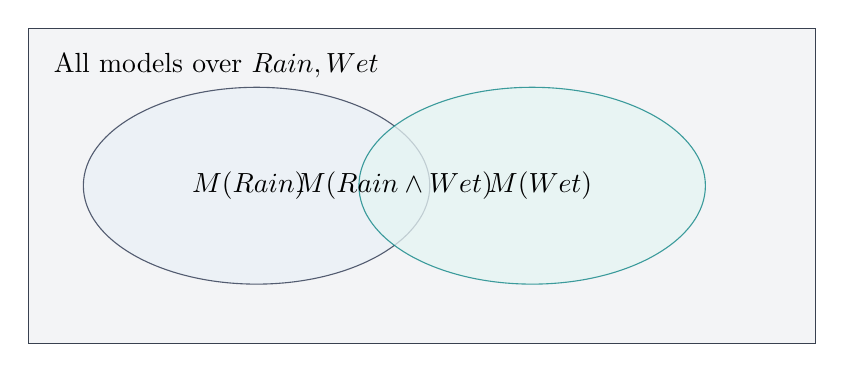
\begin{tikzpicture}
      \draw[fill=softgrey,draw=darkgrey] (0,0) rectangle (10,4);
      \node[anchor=north west] at (0.2,3.8) {All models over $Rain,Wet$};
      \draw[fill=softblue,draw=unswblue,opacity=0.75] (2.9,2) ellipse (2.2 and 1.25);
      \draw[fill=softteal,draw=unswteal,opacity=0.75] (6.4,2) ellipse (2.2 and 1.25);
      \node at (2.8,2) {$M(Rain)$};
      \node at (6.5,2) {$M(Wet)$};
      \node at (4.65,2) {$M(Rain \land Wet)$};
    \end{tikzpicture}
  \end{center}

  \begin{itemize}
    \item $M(f)$ is the set of models where formula $f$ is true.
    \item A KB is a set of formulas, so $M(KB)$ is the intersection of their model sets.
  \end{itemize}
\end{frame}

\begin{frame}{Adding Knowledge Shrinks Possibility}
  \begin{center}
    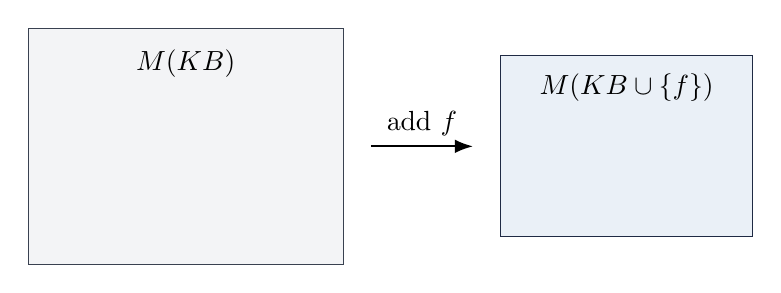
\begin{tikzpicture}[>=Latex]
      \draw[fill=softgrey,draw=darkgrey] (0,0) rectangle (4,3);
      \node at (2,2.55) {$M(KB)$};
      \draw[fill=softblue,draw=unswblue] (6,0.35) rectangle (9.2,2.65);
      \node at (7.6,2.25) {$M(KB \cup \{f\})$};
      \draw[->,thick] (4.35,1.5) -- node[above]{add $f$} (5.65,1.5);
    \end{tikzpicture}
  \end{center}

  \[
    M(KB \cup \{f\}) = M(KB) \cap M(f)
  \]

  Adding a fact can rule out worlds. It can never add new possible worlds.
\end{frame}

\begin{frame}{Entailment}
  \begin{center}
    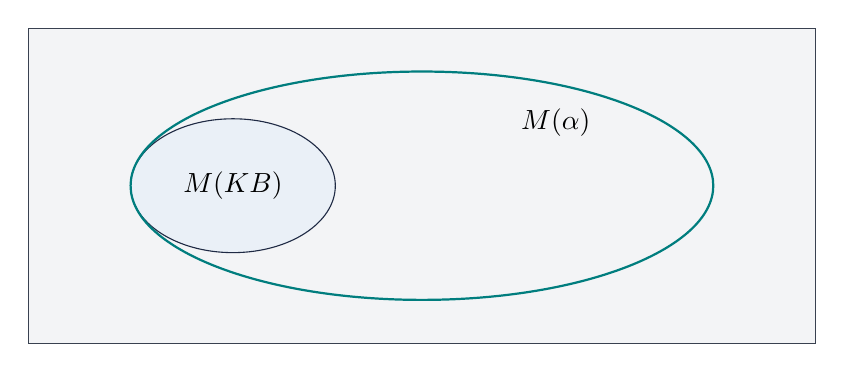
\begin{tikzpicture}
      \draw[fill=softgrey,draw=darkgrey] (0,0) rectangle (10,4);
      \draw[fill=softblue,draw=unswblue] (2.6,2) ellipse (1.3 and 0.85);
      \draw[draw=unswteal,thick] (5.0,2) ellipse (3.7 and 1.45);
      \node at (2.6,2) {$M(KB)$};
      \node at (6.7,2.8) {$M(\alpha)$};
    \end{tikzpicture}
  \end{center}

  \[
    KB \models \alpha
    \quad \text{iff} \quad
    M(KB) \subseteq M(\alpha)
  \]

  Entailment means: every world that satisfies the KB also satisfies the query.
\end{frame}

\begin{frame}{Model Checking Entailment}
  \small
  \begin{tabular}{>{\ttfamily}c>{\ttfamily}c>{\ttfamily}c|c|c}
    \toprule
    A & B & C & KB true? & Query $C$ true? \\
    \midrule
    F & F & F & no & F \\
    F & F & T & no & T \\
    F & T & F & no & F \\
    F & T & T & no & T \\
    T & F & F & no & F \\
    T & F & T & no & T \\
    T & T & F & no & F \\
    T & T & T & yes & T \\
    \bottomrule
  \end{tabular}

  \vspace{0.8em}
  For $KB = \{A,\; A \rightarrow B,\; B \rightarrow C\}$, model checking asks:

  \[
    \text{in every model where KB is true, is } C \text{ true?}
  \]

  It is sound and complete, but exponential in the number of symbols.
\end{frame}

\begin{frame}{Checkpoint: Entailment}
  \activity

  \vspace{0.5em}
  Let
  \[
    KB = \{Rain,\; Rain \rightarrow Wet\}.
  \]

  Which query is entailed by $KB$?

  \begin{itemize}
    \item \choice{A}{$Wet$}
    \item \choice{B}{$Rain \lor Snow$}
    \item \choice{C}{$Snow$}
    \item \choice{D}{A and B}
  \end{itemize}
\end{frame}

\begin{frame}{Checkpoint Answer: A And B}
  \activity

  Correct answer: \textbf{D}.

  \begin{itemize}
    \item $Wet$ is entailed by modus ponens.
    \item $Rain \lor Snow$ is entailed because $Rain$ is already true in every KB model.
    \item $Snow$ is not entailed. The KB allows worlds where $Snow$ is false.
  \end{itemize}

  Entailment can include formulas that are not the most operationally useful ones.
\end{frame}

\section{Inference}

\begin{frame}{Inference: Two Big Approaches}
  \begin{columns}[T,onlytextwidth]
    \begin{column}{0.48\textwidth}
      \minihead{Model checking}
      \begin{itemize}
        \item Enumerate or search possible worlds.
        \item Check whether all KB worlds satisfy the query.
        \item Clear semantics.
        \item Often exponential.
      \end{itemize}
    \end{column}
    \begin{column}{0.48\textwidth}
      \minihead{Theorem proving}
      \begin{itemize}
        \item Apply inference rules to formulas.
        \item Search for a proof.
        \item Avoids enumerating every model explicitly.
        \item Needs soundness and completeness guarantees.
      \end{itemize}
    \end{column}
  \end{columns}

  \source{Berkeley CS188 lecture 8; AIMA chapter 7; CS221 inference-rule slides.}
\end{frame}

\begin{frame}{Soundness And Completeness}
  \begin{columns}[T,onlytextwidth]
    \begin{column}{0.47\textwidth}
      \conceptbox{unswteal}{0.92\linewidth}{
        \minihead{Soundness}

        Everything the algorithm proves is actually entailed.

        \[
          KB \vdash \alpha \Rightarrow KB \models \alpha
        \]
      }
    \end{column}
    \begin{column}{0.47\textwidth}
      \conceptbox{unsworange}{0.92\linewidth}{
        \minihead{Completeness}

        Everything that is entailed can be proved by the algorithm.

        \[
          KB \models \alpha \Rightarrow KB \vdash \alpha
        \]
      }
    \end{column}
  \end{columns}

  \vspace{0.8em}
  We want proof procedures that match semantic entailment, not just procedures that produce formulas.
\end{frame}

\begin{frame}{Modus Ponens}
  \small
  \[
    \frac{p_1,\ldots,p_k,\quad (p_1 \land \cdots \land p_k) \rightarrow q}{q}
  \]

  \begin{columns}[T,onlytextwidth]
    \begin{column}{0.48\textwidth}
      \minihead{Example}
      \[
        \frac{Wet,\; Weekday,\; Wet \land Weekday \rightarrow Traffic}{Traffic}
      \]
    \end{column}
    \begin{column}{0.48\textwidth}
      \minihead{Role}
      \begin{itemize}
        \item Workhorse of rule-based reasoning.
        \item Sound for propositional logic.
        \item Complete only under restrictions, such as Horn clauses.
      \end{itemize}
    \end{column}
  \end{columns}

  \source{CS221 inference-rule and modus-ponens material; AIMA chapter 7.}
\end{frame}

\begin{frame}{Horn And Definite Clauses}
  \begin{columns}[T,onlytextwidth]
    \begin{column}{0.47\textwidth}
      \minihead{Definite clause}
      \[
        (p_1 \land \cdots \land p_k) \rightarrow q
      \]

      Exactly one positive conclusion.

      \medskip
      Example:
      \[
        Rain \land Snow \rightarrow Traffic
      \]
    \end{column}
    \begin{column}{0.49\textwidth}
      \minihead{As a clause}
      \[
        \neg p_1 \lor \cdots \lor \neg p_k \lor q
      \]

      Horn clauses have at most one positive literal.

      \medskip
      This restriction buys efficient chaining.
    \end{column}
  \end{columns}
\end{frame}

\begin{frame}{Forward Chaining}
  \begin{columns}[T,onlytextwidth]
    \begin{column}{0.50\textwidth}
      \minihead{Idea}
      \begin{itemize}
        \item Start with known facts.
        \item Fire rules whose premises are all known.
        \item Add their conclusions.
        \item Stop when the query is found or no new facts appear.
      \end{itemize}
    \end{column}
    \begin{column}{0.46\textwidth}
      \minihead{Office robot}
      \[
      \begin{aligned}
        K &\rightarrow \neg L\\
        \neg L &\rightarrow S\\
        P \land S &\rightarrow D\\
        K,\;P
      \end{aligned}
      \]
      Query: $D$.
    \end{column}
  \end{columns}

  \source{Berkeley CS188 lecture 8; AIMA chapter 7.}
\end{frame}

\begin{frame}{Forward Chaining Trace}
  \begin{center}
    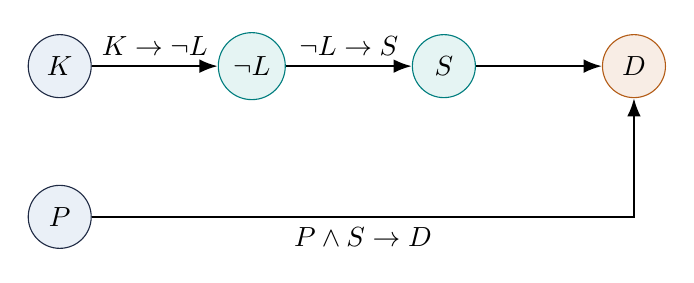
\begin{tikzpicture}[node distance=1.1cm,>=Latex]
      \node[draw=unswblue,fill=softblue,circle,minimum size=8mm] (k) {$K$};
      \node[draw=unswblue,fill=softblue,circle,minimum size=8mm,below=of k] (p) {$P$};
      \node[draw=unswteal,fill=softteal,circle,minimum size=8mm,right=1.6cm of k] (nl) {$\neg L$};
      \node[draw=unswteal,fill=softteal,circle,minimum size=8mm,right=1.6cm of nl] (s) {$S$};
      \node[draw=unsworange,fill=softorange,circle,minimum size=8mm,right=1.6cm of s] (d) {$D$};
      \draw[->,thick] (k) -- node[above]{$K\rightarrow\neg L$} (nl);
      \draw[->,thick] (nl) -- node[above]{$\neg L\rightarrow S$} (s);
      \draw[->,thick] (s) -- (d);
      \draw[->,thick] (p) -| node[pos=0.25,below]{$P\land S\rightarrow D$} (d);
    \end{tikzpicture}
  \end{center}

  \[
    \{K,P\}
    \Rightarrow \{K,P,\neg L\}
    \Rightarrow \{K,P,\neg L,S\}
    \Rightarrow \{K,P,\neg L,S,D\}
  \]

  Since $D$ is derived, forward chaining proves the query for this Horn-style KB.
\end{frame}

\begin{frame}{Forward Chaining Properties}
  \begin{itemize}
    \item Sound: every derived fact follows by sound modus ponens.
    \item Complete for definite-clause KBs: if an atomic query follows, forward chaining derives it.
    \item Linear-time implementations are possible with:
      \begin{itemize}
        \item an agenda of known facts;
        \item rule counts for remaining unsatisfied premises;
        \item indexes from symbols to rules they appear in.
      \end{itemize}
  \end{itemize}

  \vspace{0.7em}
  This is efficient because each symbol only needs to be added once.

  \source{Berkeley CS188 lecture 8 and AIMA chapter 7 forward chaining slides.}
\end{frame}

\begin{frame}{Backward Chaining}
  \begin{columns}[T,onlytextwidth]
    \begin{column}{0.48\textwidth}
      \minihead{Idea}
      \begin{itemize}
        \item Start with the query.
        \item Find rules that could conclude it.
        \item Recursively prove their premises.
        \item Stop if a subgoal is already known.
      \end{itemize}
    \end{column}
    \begin{column}{0.48\textwidth}
      \minihead{When useful}
      \begin{itemize}
        \item Goal-directed reasoning.
        \item Avoids irrelevant forward consequences.
        \item Natural for diagnostic or query-driven systems.
      \end{itemize}
    \end{column}
  \end{columns}

  \vspace{0.6em}
  Today we use it mainly to frame the limits of Horn-clause reasoning.
\end{frame}

\begin{frame}{Checkpoint: Why Horn Clauses Are Limited}
  \activity

  \vspace{0.4em}
  Which formula is \textbf{not} a definite clause?

  \begin{itemize}
    \item \choice{A}{$Rain \rightarrow Wet$}
    \item \choice{B}{$Wet \land Weekday \rightarrow Traffic$}
    \item \choice{C}{$DoorOpen$}
    \item \choice{D}{$Alarm \rightarrow Smoke \lor BreakIn$}
  \end{itemize}
\end{frame}

\begin{frame}{Checkpoint Answer: Disjunctive Conclusion}
  \activity

  Correct answer: \textbf{D}.

  \[
    Alarm \rightarrow Smoke \lor BreakIn
  \]

  A definite clause has a single atomic conclusion. A disjunctive conclusion needs a more general proof method.

  \vspace{0.8em}
  Resolution handles arbitrary clauses, not just Horn-style rules.
\end{frame}

\section{CNF And Satisfiability}

\begin{frame}{Satisfiability Connects Semantics To Algorithms}
  \begin{columns}[T,onlytextwidth]
    \begin{column}{0.48\textwidth}
      \minihead{Definitions}
      \begin{itemize}
        \item Valid: true in every model.
        \item Satisfiable: true in at least one model.
        \item Unsatisfiable: true in no model.
      \end{itemize}
    \end{column}
    \begin{column}{0.48\textwidth}
      \minihead{Examples}
      \[
      \begin{aligned}
        A \lor \neg A &\quad \text{valid}\\
        A \lor B &\quad \text{satisfiable}\\
        A \land \neg A &\quad \text{unsatisfiable}
      \end{aligned}
      \]
    \end{column}
  \end{columns}

  \source{AIMA chapter 7; Berkeley CS188 lecture 8; Basel handout.}
\end{frame}

\begin{frame}{Entailment As Unsatisfiability}
  \[
    KB \models \alpha
    \quad \text{iff} \quad
    KB \land \neg \alpha \text{ is unsatisfiable}
  \]

  \begin{columns}[T,onlytextwidth]
    \begin{column}{0.48\textwidth}
      \minihead{Why}
      \begin{itemize}
        \item If $KB$ entails $\alpha$, there is no KB-world where $\alpha$ is false.
        \item So $KB$ together with $\neg \alpha$ has no model.
      \end{itemize}
    \end{column}
    \begin{column}{0.48\textwidth}
      \minihead{Operational recipe}
      \begin{enumerate}
        \item Add the negated query.
        \item Convert everything to CNF.
        \item Try to derive contradiction.
      \end{enumerate}
    \end{column}
  \end{columns}

  \source{Berkeley CS188 lecture 8; Basel handout; AIMA chapter 7.}
\end{frame}

\begin{frame}{Conjunctive Normal Form}
  \begin{center}
    \[
      (A \lor B \lor \neg C)
      \land
      (\neg B \lor D)
      \land
      (C)
    \]
  \end{center}

  \begin{columns}[T,onlytextwidth]
    \begin{column}{0.48\textwidth}
      \minihead{CNF formula}
      \begin{itemize}
        \item conjunction of clauses;
        \item each clause is a disjunction of literals;
        \item each literal is a symbol or negated symbol.
      \end{itemize}
    \end{column}
    \begin{column}{0.48\textwidth}
      \minihead{Clause-set view}
      \[
        \{\{A,B,\neg C\},\{\neg B,D\},\{C\}\}
      \]

      This is the representation resolution operates on.
    \end{column}
  \end{columns}
\end{frame}

\begin{frame}{CNF Conversion Rules}
  \small
  \begin{tabular}{>{\bfseries}p{0.30\linewidth}p{0.55\linewidth}}
    \toprule
    Step & Rewrite \\
    \midrule
    Eliminate biconditional & $f \leftrightarrow g \equiv (f \rightarrow g) \land (g \rightarrow f)$ \\
    Eliminate implication & $f \rightarrow g \equiv \neg f \lor g$ \\
    Move negation inward & $\neg(f \land g) \equiv \neg f \lor \neg g$ \\
    Move negation inward & $\neg(f \lor g) \equiv \neg f \land \neg g$ \\
    Remove double negation & $\neg\neg f \equiv f$ \\
    Distribute & $f \lor (g \land h) \equiv (f \lor g) \land (f \lor h)$ \\
    \bottomrule
  \end{tabular}

  \vspace{0.8em}
  These rewrites preserve models: the old formula and the new formula are equivalent.

  \source{Stanford/CS221 resolution material; Berkeley CS188 lecture 8; AIMA chapter 7.}
\end{frame}

\begin{frame}{CNF Conversion Example}
  Convert:
  \[
    (Summer \rightarrow Snow) \rightarrow Bizarre
  \]

  \[
  \begin{aligned}
    (Summer \rightarrow Snow) \rightarrow Bizarre
      &\equiv \neg(\neg Summer \lor Snow) \lor Bizarre\\
      &\equiv (Summer \land \neg Snow) \lor Bizarre\\
      &\equiv (Summer \lor Bizarre) \land (\neg Snow \lor Bizarre)
  \end{aligned}
  \]

  The final line is CNF: a conjunction of two clauses.

  \source{Adapted from Stanford/CS221 resolution material.}
\end{frame}

\begin{frame}{Checkpoint: Is This CNF?}
  \activity

  \vspace{0.4em}
  Which formula is in CNF?

  \begin{itemize}
    \item \choice{A}{$(A \land B) \lor C$}
    \item \choice{B}{$(A \lor \neg B) \land (C \lor D)$}
    \item \choice{C}{$A \rightarrow B$}
    \item \choice{D}{$\neg(A \lor B) \land C$}
  \end{itemize}
\end{frame}

\begin{frame}{Checkpoint Answer: Clause Conjunction}
  \activity

  Correct answer: \textbf{B}.

  \[
    (A \lor \neg B) \land (C \lor D)
  \]

  Each top-level part is a clause, and each clause is a disjunction of literals.

  \medskip
  D is equivalent to CNF after rewriting, but it is not already in CNF because the negation is applied to a compound formula.
\end{frame}

\begin{frame}{SAT Solvers In One Slide}
  \begin{columns}[T,onlytextwidth]
    \begin{column}{0.48\textwidth}
      \minihead{DPLL}
      \begin{itemize}
        \item Searches over partial models.
        \item Stops early when clauses are satisfied or contradicted.
        \item Uses unit propagation and pure literals.
        \item Modern SAT solvers scale this core idea aggressively.
      \end{itemize}
    \end{column}
    \begin{column}{0.48\textwidth}
      \minihead{Why mention it here}
      \begin{itemize}
        \item SAT solving is model search.
        \item Resolution is proof search.
        \item Both exploit CNF.
        \item Your local \texttt{ai9414.logic} module traces DPLL examples.
      \end{itemize}
    \end{column}
  \end{columns}

  \source{Berkeley CS188 lecture 8; local \texttt{src/ai9414/logic} examples.}
\end{frame}

\section{Resolution}

\begin{frame}{Why Resolution}
  \begin{center}
    \small
    \begin{tabular}{p{0.32\linewidth}p{0.28\linewidth}p{0.24\linewidth}}
      \toprule
      Formula class & Inference rule & Complete? \\
      \midrule
      Full propositional logic & Modus ponens & No \\
      Horn clauses only & Modus ponens & Yes \\
      Full propositional logic in CNF & Resolution & Yes, for refutation \\
      \bottomrule
    \end{tabular}
  \end{center}

  \vspace{0.8em}
  Resolution is the main proof method for this class because it handles arbitrary propositional clauses.

  \source{Stanford/CS221 resolution material; AIMA chapter 7.}
\end{frame}

\begin{frame}{Resolution Generalises The Cancellation Idea}
  \[
    \frac{Rain \lor Snow,\quad \neg Snow \lor Traffic}{Rain \lor Traffic}
  \]

  \vspace{0.5em}
  The two parent clauses disagree on $Snow$.

  \begin{center}
    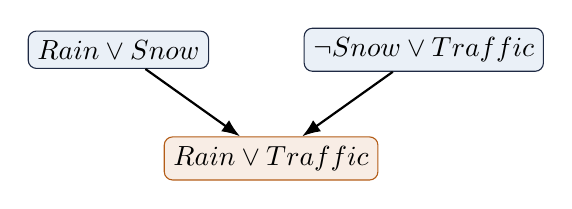
\begin{tikzpicture}[node distance=1.2cm,>=Latex]
      \node[draw=unswblue,fill=softblue,rounded corners=3pt] (a) {$Rain \lor Snow$};
      \node[draw=unswblue,fill=softblue,rounded corners=3pt,right=of a] (b) {$\neg Snow \lor Traffic$};
      \node[draw=unsworange,fill=softorange,rounded corners=3pt,below=1.1cm of $(a)!0.5!(b)$] (c) {$Rain \lor Traffic$};
      \draw[->,thick] (a) -- (c);
      \draw[->,thick] (b) -- (c);
    \end{tikzpicture}
  \end{center}

  If both parent clauses are true, the resolvent must be true.
\end{frame}

\begin{frame}{The Resolution Rule}
  \[
    \frac{f_1 \lor \cdots \lor f_n \lor p,\quad
      \neg p \lor g_1 \lor \cdots \lor g_m}
    {f_1 \lor \cdots \lor f_n \lor g_1 \lor \cdots \lor g_m}
  \]

  \begin{itemize}
    \item $p$ and $\neg p$ are complementary literals.
    \item The conclusion is the resolvent.
    \item Parent clauses are kept; the resolvent is added to the clause set.
  \end{itemize}

  \source{Stanford/CS221 resolution material; TUM resolution slides.}
\end{frame}

\begin{frame}{Clause-Set Corner Cases}
  \begin{columns}[T,onlytextwidth]
    \begin{column}{0.47\textwidth}
      \conceptbox{unsworange}{0.92\linewidth}{
        \minihead{Empty clause}

        \[
          \Box
        \]

        A disjunction over zero literals.

        It means contradiction: false.
      }
    \end{column}
    \begin{column}{0.47\textwidth}
      \conceptbox{unswteal}{0.92\linewidth}{
        \minihead{Empty set of clauses}

        \[
          \{\}
        \]

        A conjunction over zero clauses.

        It means trivially true.
      }
    \end{column}
  \end{columns}

  \source{Basel handout and TUM resolution slides.}
\end{frame}

\begin{frame}{Resolution Refutation Algorithm}
  To test $KB \models \alpha$:

  \begin{enumerate}
    \item Build $KB \land \neg \alpha$.
    \item Convert the result to CNF.
    \item Treat each CNF clause as a set of literals.
    \item Repeatedly resolve pairs of clauses.
    \item If the empty clause $\Box$ appears, return entailed.
    \item If no new clauses appear, return not entailed.
  \end{enumerate}

  \vspace{0.6em}
  This is proof by contradiction in clause form.

  \source{AIMA chapter 7 resolution algorithm; Stanford/CS221; Basel handout.}
\end{frame}

\begin{frame}{Worked Refutation: Chain Entailment}
  \begin{columns}[T,onlytextwidth]
    \begin{column}{0.46\textwidth}
      \minihead{Knowledge base}
      \[
      \begin{aligned}
        A &\rightarrow B\\
        B &\rightarrow C\\
        A
      \end{aligned}
      \]

      Query:
      \[
        C
      \]
    \end{column}
    \begin{column}{0.50\textwidth}
      \minihead{CNF for $KB \land \neg C$}
      \[
        \{\neg A \lor B,\; \neg B \lor C,\; A,\; \neg C\}
      \]

      This is the same conceptual pattern used by the local \texttt{entailment\_chain} DPLL example.
    \end{column}
  \end{columns}
\end{frame}

\begin{frame}{Worked Refutation: Proof}
  \begin{center}
    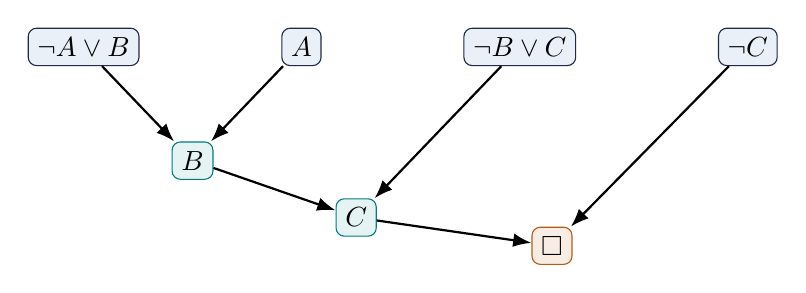
\begin{tikzpicture}[node distance=1.2cm,>=Latex]
      \node[draw=unswblue,fill=softblue,rounded corners=3pt] (c1) {$\neg A \lor B$};
      \node[draw=unswblue,fill=softblue,rounded corners=3pt,right=1.8cm of c1] (c2) {$A$};
      \node[draw=unswteal,fill=softteal,rounded corners=3pt,below=of $(c1)!0.5!(c2)$] (r1) {$B$};

      \node[draw=unswblue,fill=softblue,rounded corners=3pt,right=1.8cm of c2] (c3) {$\neg B \lor C$};
      \node[draw=unswteal,fill=softteal,rounded corners=3pt,below=of $(r1)!0.5!(c3)$] (r2) {$C$};

      \node[draw=unswblue,fill=softblue,rounded corners=3pt,right=1.8cm of c3] (c4) {$\neg C$};
      \node[draw=unsworange,fill=softorange,rounded corners=3pt,below=of $(r2)!0.5!(c4)$] (bot) {$\Box$};

      \draw[->,thick] (c1) -- (r1);
      \draw[->,thick] (c2) -- (r1);
      \draw[->,thick] (r1) -- (r2);
      \draw[->,thick] (c3) -- (r2);
      \draw[->,thick] (r2) -- (bot);
      \draw[->,thick] (c4) -- (bot);
    \end{tikzpicture}
  \end{center}

  \[
    KB \land \neg C \vdash \Box
    \quad \Rightarrow \quad
    KB \models C
  \]
\end{frame}

\begin{frame}{Worked Refutation: Disjunctive Example}
  \[
    KB = \{A \rightarrow (B \lor C),\; A,\; \neg B,\; \neg C\}
  \]

  Convert:
  \[
    \{\neg A \lor B \lor C,\; A,\; \neg B,\; \neg C\}
  \]

  \begin{center}
    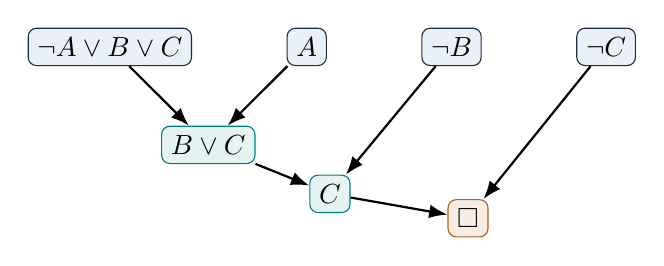
\begin{tikzpicture}[node distance=1cm,>=Latex]
      \node[draw=unswblue,fill=softblue,rounded corners=3pt] (a) {$\neg A \lor B \lor C$};
      \node[draw=unswblue,fill=softblue,rounded corners=3pt,right=1.2cm of a] (b) {$A$};
      \node[draw=unswteal,fill=softteal,rounded corners=3pt,below=of $(a)!0.5!(b)$] (bc) {$B \lor C$};
      \node[draw=unswblue,fill=softblue,rounded corners=3pt,right=1.2cm of b] (nb) {$\neg B$};
      \node[draw=unswteal,fill=softteal,rounded corners=3pt,below=of $(bc)!0.5!(nb)$] (c) {$C$};
      \node[draw=unswblue,fill=softblue,rounded corners=3pt,right=1.2cm of nb] (nc) {$\neg C$};
      \node[draw=unsworange,fill=softorange,rounded corners=3pt,below=of $(c)!0.5!(nc)$] (bot) {$\Box$};
      \draw[->,thick] (a) -- (bc);
      \draw[->,thick] (b) -- (bc);
      \draw[->,thick] (bc) -- (c);
      \draw[->,thick] (nb) -- (c);
      \draw[->,thick] (c) -- (bot);
      \draw[->,thick] (nc) -- (bot);
    \end{tikzpicture}
  \end{center}

  This is the Stanford-style example showing why resolution is useful beyond Horn chaining.
\end{frame}

\begin{frame}{Resolution Is Sound}
  If both clauses are true:

  \[
    (Rain \lor Snow) \land (\neg Snow \lor Traffic)
  \]

  then one of these cases must hold:

  \begin{itemize}
    \item $Snow$ is true, so the second clause forces $Traffic$.
    \item $Snow$ is false, so the first clause forces $Rain$.
  \end{itemize}

  Therefore:

  \[
    Rain \lor Traffic
  \]

  must be true. The resolvent is entailed by the parent clauses.
\end{frame}

\begin{frame}{Resolution Is Complete For Refutation}
  \begin{itemize}
    \item Resolution is not a magic way to derive every consequence directly.
    \item Its key guarantee is refutation completeness:
  \end{itemize}

  \[
    \Delta \text{ is unsatisfiable}
    \quad \text{iff} \quad
    \Delta \vdash_{Res} \Box
  \]

  \vspace{0.8em}
  To prove $KB \models \alpha$, do not try to derive $\alpha$ directly.

  \[
    \text{Prove } KB \cup \{\neg \alpha\} \vdash_{Res} \Box.
  \]

  \source{TUM resolution slides; Basel handout; Stanford/CS221 resolution material.}
\end{frame}

\begin{frame}{What Resolution Costs}
  \begin{columns}[T,onlytextwidth]
    \begin{column}{0.48\textwidth}
      \minihead{Good news}
      \begin{itemize}
        \item Sound.
        \item Refutation-complete for propositional logic.
        \item One uniform rule.
        \item Works after CNF conversion.
      \end{itemize}
    \end{column}
    \begin{column}{0.48\textwidth}
      \minihead{Bad news}
      \begin{itemize}
        \item Naive resolution can generate many clauses.
        \item Worst-case proofs can be exponential.
        \item Practical systems need good strategies.
      \end{itemize}
    \end{column}
  \end{columns}

  \vspace{0.6em}
  This trade-off mirrors the move from efficient Horn reasoning to full propositional expressiveness.
\end{frame}

\begin{frame}{Checkpoint: One Resolution Step}
  \activity

  \vspace{0.4em}
  Resolve:

  \[
    A \lor B \lor \neg C
    \qquad
    C \lor D
  \]

  on $C$. What is the resolvent?

  \begin{itemize}
    \item \choice{A}{$A \lor B \lor D$}
    \item \choice{B}{$A \lor B \lor \neg C \lor C \lor D$}
    \item \choice{C}{$A \lor B$}
    \item \choice{D}{$D$}
  \end{itemize}
\end{frame}

\begin{frame}{Checkpoint Answer: Remove Complementary Literals}
  \activity

  Correct answer: \textbf{A}.

  \[
    \frac{A \lor B \lor \neg C,\quad C \lor D}{A \lor B \lor D}
  \]

  The complementary pair is $\neg C$ and $C$.

  Keep the remaining literals from both clauses.
\end{frame}

\begin{frame}{Checkpoint: Does The Refutation Prove Entailment?}
  \activity

  \vspace{0.4em}
  We want to test whether $KB \models Q$.

  After adding $\neg Q$ and converting to CNF, resolution derives $\Box$.

  What should we conclude?

  \begin{itemize}
    \item \choice{A}{$KB \models Q$}
    \item \choice{B}{$KB \models \neg Q$}
    \item \choice{C}{$KB$ is satisfiable and says nothing about $Q$}
    \item \choice{D}{Resolution has failed}
  \end{itemize}
\end{frame}

\begin{frame}{Checkpoint Answer: The Query Is Entailed}
  \activity

  Correct answer: \textbf{A}.

  \[
    KB \land \neg Q \vdash \Box
  \]

  means there is no model where $KB$ is true and $Q$ is false.

  Therefore every model of $KB$ is a model of $Q$.
\end{frame}

\section{Short FOL Preview}

\begin{frame}{Where Propositional Logic Runs Out}
  \begin{columns}[T,onlytextwidth]
    \begin{column}{0.50\textwidth}
      \minihead{Propositional encoding}
      \[
      \begin{aligned}
        SafeA,\; SafeB,\; SafeC,\ldots\\
        HasKeyAlice,\; HasKeyBob,\ldots
      \end{aligned}
      \]

      Each object-specific fact needs its own symbol.
    \end{column}
    \begin{column}{0.46\textwidth}
      \minihead{Problem}
      \begin{itemize}
        \item Cannot talk compactly about many objects.
        \item Cannot state general rules over all rooms or people.
        \item New objects require new propositional symbols and rules.
      \end{itemize}
    \end{column}
  \end{columns}

  \source{AIMA chapter 7 summary: propositional logic lacks expressive power.}
\end{frame}

\begin{frame}{First-Order Logic Preview}
  \begin{columns}[T,onlytextwidth]
    \begin{column}{0.48\textwidth}
      \minihead{What FOL adds}
      \begin{itemize}
        \item objects;
        \item predicates;
        \item variables;
        \item quantifiers.
      \end{itemize}
    \end{column}
    \begin{column}{0.48\textwidth}
      \minihead{Example}
      \[
        \forall x\; HasKey(x) \rightarrow CanEnter(x,Lab)
      \]

      One sentence can describe a whole family of propositional cases.
    \end{column}
  \end{columns}

  \vspace{0.8em}
  FOL inference is a later topic. Today the proof method to master is propositional resolution.
\end{frame}

\begin{frame}{What To Remember}
  \begin{enumerate}
    \item Propositional logic represents knowledge as formulas over true/false symbols.
    \item Entailment is semantic: all KB models satisfy the query.
    \item Inference is syntactic: rules derive new formulas.
    \item Soundness and completeness connect proof to truth.
    \item Horn-clause chaining is efficient but restricted.
    \item CNF makes clauses explicit.
    \item Resolution proves entailment by refuting $KB \land \neg query$.
    \item Propositional logic is useful, but not compact enough for rich object domains.
  \end{enumerate}
\end{frame}

\begin{frame}{End-Of-Class Worked Problem}
  \small
  \[
  KB =
  \{
    A \rightarrow B,\;
    A \rightarrow C,\;
    B \land C \rightarrow D,\;
    D \rightarrow E,\;
    A
  \}
  \]

  \[
    \text{Query: } E
  \]

  \begin{columns}[T,onlytextwidth]
    \begin{column}{0.48\textwidth}
      \minihead{Task 1}
      Prove $E$ using forward chaining.
    \end{column}
    \begin{column}{0.48\textwidth}
      \minihead{Task 2}
      Convert $KB \land \neg E$ to CNF clauses and outline a resolution refutation.
    \end{column}
  \end{columns}

  \vspace{0.8em}
  This is the final synthesis: one semantic claim, two proof styles.
\end{frame}

\begin{frame}{Worked Problem Solution Sketch}
  \begin{columns}[T,onlytextwidth]
    \begin{column}{0.46\textwidth}
      \minihead{Forward chaining}
      \[
        A \Rightarrow B,\; C
      \]
      \[
        B,C \Rightarrow D
      \]
      \[
        D \Rightarrow E
      \]
    \end{column}
    \begin{column}{0.50\textwidth}
      \minihead{Resolution clauses}
      \[
      \begin{aligned}
        &\neg A \lor B,\quad \neg A \lor C,\quad \neg B \lor \neg C \lor D,\\
        &\neg D \lor E,\quad A,\quad \neg E
      \end{aligned}
      \]

      Resolve to get $B$, $C$, $D$, $E$, then resolve $E$ with $\neg E$ to derive $\Box$.
    \end{column}
  \end{columns}
\end{frame}

\appendix
\section{Appendix}

\begin{frame}{Primary Local Sources}
  \small
  \begin{itemize}
    \item Berkeley CS188 lecture 8, \textit{Inference in Propositional Logic}: \texttt{0-material/cs188-sp24-lec08.pdf}.
    \item AIMA chapter 7, \textit{Logical Agents}: \texttt{0-material/chapter07.pdf}.
    \item Stanford/CS221-style resolution material: \texttt{0-material/propositional-resolution.pdf}.
    \item Basel 2025 handout, \textit{Propositional Logic: Reasoning and Resolution}: \texttt{0-material/ai-e03-handout4.pdf}.
    \item TUM propositional resolution slides: \texttt{0-material/resolution-prop.pdf}.
    \item Supplementary CS221-style PDFs: syntax, semantics, inference rules, modus ponens.
  \end{itemize}
\end{frame}

\begin{frame}{Optional Whiteboard Prompts}
  \begin{itemize}
    \item Draw the model-set inclusion picture for $KB \models \alpha$.
    \item Ask students to invent a model where $KB$ is true and a non-entailed query is false.
    \item Convert $B_{1,1} \leftrightarrow (P_{1,2} \lor P_{2,1})$ to CNF.
    \item Resolve $\{P,Q\}$, $\{P,\neg Q\}$, $\{\neg P,Q\}$, $\{\neg P,\neg Q\}$ to contradiction.
    \item Ask which step proves the query: deriving the query directly, or deriving $\Box$ after adding its negation.
  \end{itemize}
\end{frame}

\end{document}
